\chapter[Topic: Determinants of Interest Rates]{Topic: Determinants of Interest Rates (0-10\%)}

\subsection{Information}

\begin{distributions}[Objective]
The Candidate will understand key concepts concerning the determinants of interest rates, the components of interest, and how to perform related calculations.
\end{distributions}

\begin{outcomes}[Learning outcomes]
The candidate will be able to:
\begin{enumerate}[label = \alph*), leftmargin = *]
	\item	Define and recognize the \textit{definitions} of the following terms:
		\begin{itemize}[leftmargin = *]
		\item	Real risk-free rate;
		\item	Inflation rate;
		\item	Default risk premium;
		\item	Liquidity premium;
		\item	Maturity risk premium.
		\end{itemize}
	\item	Explain how the components of interest rates apply in various contexts, such as:
		\begin{itemize}[leftmargin = *]
		\item	Commercial loans;
		\item	Mortgages;
		\item	Credit cards;
		\item	Bonds;
		\item	Government securities.
		\end{itemize}
	\item	Explain the \textbf{roles} of the Federal Reserve and the FOMC in carrying out \textit{fiscal} policy and \textit{monetary} policy and the \textbf{tools} used thereby including:
		\begin{itemize}[leftmargin = *]
		\item	Targeting the federal funds rate;
		\item	Setting reserve requirements;
		\item	Setting the discount rate.
		\end{itemize}
	\item	Explain the theories of why interest rates differ by term, including :
		\begin{itemize}[leftmargin = *]
		\item	Liquidity preference (opportunity cost);
		\item	Expectations;
		\item	Preferred habitat; 
		\item	Market segmentation.
		\end{itemize}
	\item	Explain how interest rates differ from one country to another (e.g., U.S. vs. Canada);
	\item	In the context of loans with and without inflation protection:
		\begin{itemize}[leftmargin = *]
		\item	\textbf{Identify} the \textit{real} interest and the \textit{nominal} interest rate;
		\item	\textbf{Calculate} the effect of changes in inflation on loans with inflation protection.
		\end{itemize}
\end{enumerate}
\end{outcomes}

\begin{ASM_chapter}[Related lessons ASM]
Section 9: Determinants of Interest Rates
\begin{itemize}[leftmargin = *]
	\item	\nameref{L.-9a}
	\item	\nameref{L.-9b}
	\item	\nameref{L.-9c}
	\item	\nameref{L.-9d}
	\item	\nameref{L.-9e}
	\item	\nameref{L.-9f}
	\item	\nameref{L.-9g}
	\item	\nameref{L.-9h}
	\item	\nameref{L.-9i}
\end{itemize}
\end{ASM_chapter}

\subsection{Chapter summaries}

\begin{CHPT_SUMM_AUTO}[label = {L.-9a}]{9a. What is Interest?}
From an economic perspective, can view interest in one of two ways:
\begin{itemize}
	\item	Compensation for deferring consumption (e.g., putting money in a savings account rather than spending it).
	\item	Cost of consuming resources which aren't available (e.g., using a credit card to buy something).
\end{itemize}
People's choices will vary based on this consumption; if interest rates (the compensation) are high, more people will tend to save rather than spend. The demand curve is based on this.

\end{CHPT_SUMM_AUTO}

\begin{CHPT_SUMM_AUTO}[label = {L.-9b}]{9b. Quotation Bases for Interest Rates}
\begin{description}
	\item[$d$]	quoted rate.
	\item[$N$]	Number of days to maturity.
	\item[$P$]	Price at issue.
	\item[$C$]	Maturity value.
	\item[$\textcolor{teal}{I}$]	Amount of interest earned = $\textcolor{teal}{C - P}$
\end{description}
Quoted rate of US T-bills $\frac{360}{N}\times \frac{\textcolor{teal}{C - P}}{C}$. 
\begin{itemize}[leftmargin = *]
	\item	This rate is very simple to calculate and in the 1930s was much easier.
	\item	Thus, even if the compound rate $P_{t} = P_{0}(1 + i)^{t}$ is a more accurate representation of the rate of growth, the quoted rate is used.
\end{itemize}
Quoted rate of Canadian Government T-Bills is $\frac{365}{N}\times \frac{\textcolor{teal}{C - P}}{P}$. 
\begin{itemize}[leftmargin = *]
	\item	Thus we compare to the price and assume 365 days instead of 360.
\end{itemize}

To minimize mistakes, it is good practice to convert all interest rates to a common basis.
\begin{description}
	\item[Effective interest rate]	The rate $i$ defined by $P_{t} = P_{0}(1 + i)^{t}$.
	\item[Effective per annum interest rate]	Special case of the above when $t$ is measured in years.
		\begin{itemize}[leftmargin = *]
		\item	Note this is not the \textbf{constant} rate and as such a function of $t$ shouldn't be powered to an exposant but multiplied.
		\end{itemize}
	\item[Continuously compounded rate]	The rate $r$ defined by $P_{t} = P_{0} \textrm{e}^{rt}$.
	\item[Continuously compounded per annum rate]	Special case of the above when $t$ is measured in years.
		\begin{itemize}[leftmargin = *]
		\item	Note this is not the \textbf{constant} rate and as such a function of $t$ shouldn't be integrated but summed.
		\end{itemize}
\end{description}
Unlike effective rates, continuous ones are additive and easier to work with. 
\end{CHPT_SUMM_AUTO}

\begin{CHPT_SUMM_AUTO}[label = {L.-9c}]{9c. Components of the Interest Rate: No Inflation or Default Risk}
\paragraph{Market segmentation theory}
\begin{itemize}[leftmargin = *]
	\item	People interested in borrowing money for the short and long term are different.
		\begin{itemize}[leftmargin = *]
		\item	In the short-term, people may have a cash shortfall but expect to earn enough money to repay the loan by the end of the year.
		\item	In the long-term, people may be starting a business and expect to repay the loan in a few years.
		\end{itemize}
	\item	The same idea holds for the lenders.
		\begin{itemize}[leftmargin = *]
		\item	In the short-term, people are saving money for a short-term goal and need access to their money relatively soon.
		\item	In the long-term, people may be saving for retirement and don't mind not having immediate access to their money for a long time.
		\end{itemize}
\end{itemize}

\paragraph{The opportunity cost, or liquidity preference, theory}
\begin{itemize}[leftmargin = *]
	\item	Ceteris Paribus, lenders tend to prefer to lend money for shorter terms.
	\item	Thus, borrows generally have to pay a higher rate of interest, not just higher compensation, to persuade lenders to lend money for longer.
\end{itemize}

\paragraph{Expectations theory}
\begin{itemize}[leftmargin = *]
	\item	Interest rates on longer term loans provide information on the future expected rate of shorter term loans.
\end{itemize}

\paragraph{Preferred habitat theory}
\begin{itemize}[leftmargin = *]
	\item	Similarly to the market segmentation theory, differences in rates are due to differences in the pools of lenders / borrowers.
	\item	However, lenders / borrowers are \textbf{not rigidly segmented} by term.
\end{itemize}

\tcbline

\paragraph{Yield Curve}	Collection of interest rate values for the different terms (\textit{spot rates})
\begin{center}
	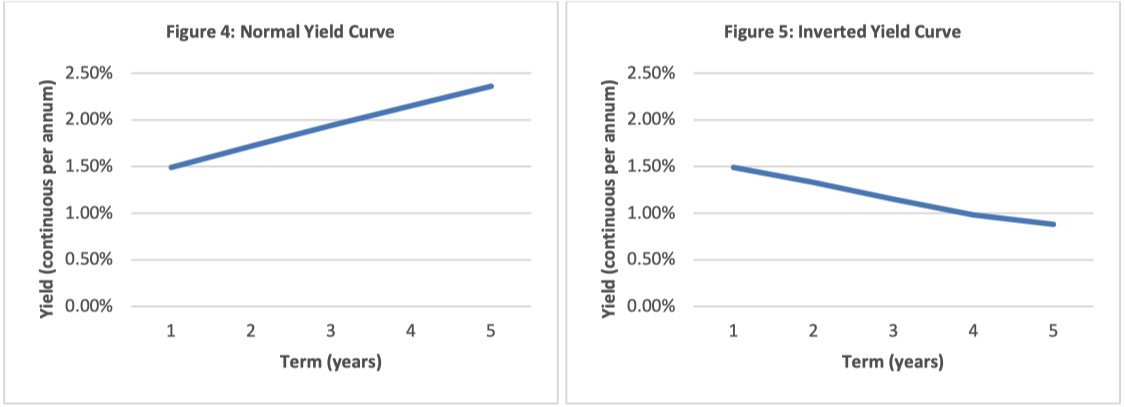
\includegraphics[scale=0.3]{img/yield-curve-2.png}
	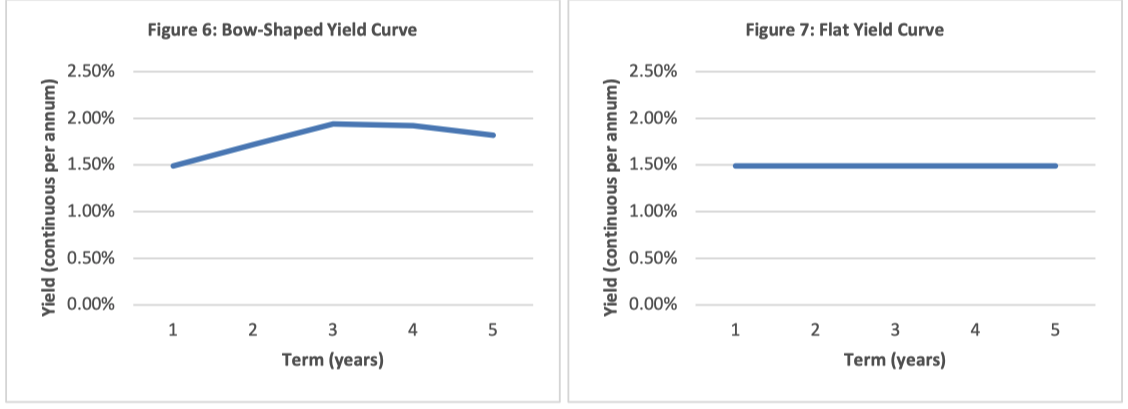
\includegraphics[scale=0.3]{img/yield-curve.png}
\end{center}
\end{CHPT_SUMM_AUTO}

\begin{CHPT_SUMM_AUTO}[label = {L.-9d}]{9d. Components of the Interest Rate: no Inflation but with Default Risk}
\paragraph{Notation for problems involving defaults (amounts)}
\begin{description}
	\item[$x$]	Amount received from every borrower (assuming no defaults).
	\item[$y$]	Amount received from every borrower who does not default (assuming defaults at rate $q$).
	\item[$q$]	Rate of default, expressed either as a decimal or a percentage of all borrowers.
	\item[$p$]	Fraction of the recoveries received from those who default at the end of the loan term.
\end{description}

\paragraph{when there is default with}
\begin{description}
	\item[no recovery]	The lender requires:
		\[
			x = (1 - q)y
		\]
	\item[partial recovery of $p$]	The lender requires :
		\[
			x = (1 - q)y + qpy \equiv [1 - (1 - p)q]y
		\]
\end{description}

\tcbline

\paragraph{Notation for problems involving defaults (rates)}
\begin{description}
	\item[$R$]	Rate on the loan with default risk.
	\item[$r$]	Rate on the (same term) loan without default risk.
		\begin{itemize}[leftmargin = *]
		\item	In other words, the \textit{compensation for deferred risk}.
		\end{itemize}
	\item[$s$]	When continuous it is the difference between the two rates, 	\\
				when effective it is the \textit{compensation for default risk}.		
\end{description}
\begin{itemize}[leftmargin = *]
	\item	When rates are continuous per annum, we can decompose them as $R = r + s$.
	\item	When rates are effective per annum, we can decompose them as $1 + R = (1 + r)(1 + s)$.
	\item	When it is effective, we can approximate $R \approx r + s$. \\
			In this case, the difference between the exact and approximate $R$ is the error in ignoring the $rs$ term.
\end{itemize}
\end{CHPT_SUMM_AUTO}

\begin{CHPT_SUMM_AUTO}[label = {L.-9e}]{9e. Components of the Interest Rate: Known Inflation}
\begin{description}
	\item[Inflation]	Tendency for prices to increase over time.
		\begin{itemize}[leftmargin = *]
		\item	Usually tracked with a specific basket of goods and services.
		\item	There are \textit{consumer} price indexes (CPI) and \textit{producer} price indexes (PPI) for \textbf{domestic} products.
		\end{itemize}
	\item[Inflation Rate]	Change in the price-level of an index.
		\begin{itemize}[leftmargin = *]
		\item	Generally compounded per annum.
		\item	Provide information on the \textit{general} tendency for prices to increase.
		\end{itemize}
\end{description}
\begin{itemize}[leftmargin = *]
	\item	Inflation thus leads to lenders requiring a higher interest rate from borrowers to compensate for the \textbf{loss in purchasing power} over the term of the loan.
	\item	This is balanced by borrowers generally having a higher future income.
\end{itemize}

\begin{description}
	\item[$R$]	Equilibrium interest rate.
		\begin{itemize}[leftmargin = *]
		\item	Generally continuous per annum.
		\item	Accounts for deferred spending and default risk.
		\end{itemize}
	\item[$i$]	Certain rate of inflation per year (in both wages and price).
		\begin{itemize}[leftmargin = *]
		\item	Generally continuous per annum.
		\item	Have to be careful not to get confused with $i$ representing inflation.
		\end{itemize}
	\item[$R^{*}$]	Equilibrium rate in a world of certain inflation (also considers default risk).
		\begin{align*}
		R^{*}	&=	r + s + i, \text{continuous per annum}	\\
		1 + R^{*}	&=	(1 + r) (1 + s) (1 + i), \text{effective per annum}	\\
		\end{align*}
\end{description}
\end{CHPT_SUMM_AUTO}

\begin{CHPT_SUMM_AUTO}[label = {L.-9f}]{9f. Components of the Interest Rate: Uncertain Inflationo}
\textbf{Loans with inflation protection} preserve the lender's purchasing power but have uncertainty into the amount the borrow must ultimately repay. A borrower may be willing to pay the lender additional interest to avoid the uncertainty of payment. In this \textbf{loan without inflation protection}, the \textit{lender assumes the risk} of the purchasing power not being preserved and sets higher repayment levels.\\

\paragraph{Notation}
\begin{description}
	\item[$r$]	Compensation for deferred consumption.
	\item[$c$]	Cost of inflation protection.
	\item[$s$]	The \textbf{credit spread}, or spread for credit risk.
		\begin{itemize}[leftmargin = *]
		\item	These vary according to the terms and a collection of spreads is a \textbf{spread curve}.
		\item	In practice, this is calculated by the difference in the observed rates on the loan with and without default risk:
		\end{itemize}
		\begin{align*}
		s	&=	R^{*} - R_{2}
		\end{align*}
	\item[$i_{a}$]	Actual (realized) rate of inflation.
	\item[$i_{e}$]	Compensation for expected inflation.
		\begin{itemize}[leftmargin = *]
		\item	When there is certain inflation, i.e. $s = 0$, then $i_{e}$ is simply the expected rate of inflation $i$.
		\end{itemize}
	\item[$i_{u}$]	Compensation for unexpected inflation.
		\begin{itemize}[leftmargin = *]
		\item	When inflation rates are stable $i_{u}$, will be fairly small.\\
			 	When they're volatile, $i_{u}$ could be quite large.
		\end{itemize}
\end{description}
\begin{description}
	\item[$R_{1}$]	Quoted rate, or \textbf{real interest rate}, on a loan \textbf{with inflation protection} but no default risk.
		\begin{align*}
		R_{1}	&=	r - c
		\end{align*}
	\item[$R_{1}^{(a)}$]	Rate actually realized (loan with inflation protection).
		\begin{align*}
		R_{1}^{(a)}	&=	r - c + i_{a}
		\end{align*}
	\item[$R_{2}$]	Quoted rate, or \textbf{nominal interest rate}, on a loan \textbf{without inflation protection} and no default risk.
		\begin{align*}
		R_{2}	&=	r + i_{e} + i_{u}
		\end{align*}
	\item[$R^{*}$]	The interest rate on a loan \textbf{with risk of default}.
		\begin{align*}
		R^{*}	&=	r + s + i_{e} + i_{u}
		\end{align*}	
\end{description}

\begin{itemize}
	\item	Although $r$, $c$, $i_{e}$, and $i_{u}$ cannot be observed individually, only the rates $R_{1}$ and $R_{2}$. 
	\item	That said, we can observe $R_{2} - R_{1} = i_{e} + i_{u} - c$ which are the compensation and costs for inflation.
	\item	Financial commentators therefore often say the difference provides an indication of the inflation rate expected by the market.\\
			However, this only holds when the market is stable and $i_{u}$ is small.\\
			Thereby, the difference tends to overestimate the market's expectation of future inflation.
\end{itemize}

\paragraph{Note}	\hl{Practice some problems with inflation indexes to ensure I know how to apply the theory.}
\end{CHPT_SUMM_AUTO}

\begin{CHPT_SUMM_AUTO}[label = {L.-9g}]{9g. Savings and Lending Interest Rates}
\begin{description}
	\item[Financial intermediaries]	Third party who matches up borrowers and lenders.
		\begin{itemize}[leftmargin = *]
		\item	In retail markets these are banks as well as savings and loan companies.
		\item	They accept deposits from the general public and in turn lend to individuals and businesses.
		\item	They must therefore charge a rate greater than that paid on the deposits to cover \textbf{overhead costs} and \textbf{losses on defaults}.
		\item	Thereby, the failure of a bank can impact not only depositors, but also the economy by stopping transactions with debit and credit cards.
		\end{itemize}
	\item[Shadow banking]	Lenders who do not accept deposits from the general but instead directly from investors.
		\begin{itemize}[leftmargin = *]
		\item	Therefore, they're not regulated as banks.
		\item	Their risk and growing importance is considerable (see 2008's crash).
		\end{itemize}
	\item[Financial technology companies (fintech)]	Alternative payment providers which operate outside the traditional banking system.
		\begin{itemize}[leftmargin = *]
		\item	E.g. PayPal, Apple Pay, Bitcoin, etc.
		\end{itemize}
\end{description}

\tcbline

Banks have 2 typical savings products:
\begin{description}
	\item[Savings accounts]	Completely liquid.
	\item[Certificates of deposit (CD)]	Illiquid for a fixed period of time.
\end{description}
The rate of these can be influenced by:
\begin{itemize}[leftmargin = *]
	\item	The overhead cost of the bank.
		\begin{itemize}[leftmargin = *]
		\item	This is the main factor.
		\item	This is why online banks are cheaper, and banks in different regions may have different rates.
		\end{itemize}
	\item	Banks looking to grow may offer a higher rate on their savings products.
	\item	The credit rating of a bank can also affect it's interest rate with riskier ones having to offer a greater rate.
\end{itemize}

\tcbline

Banks have 3 basic types of lending products:
\begin{description}
	\item[Secured loans]	\textbf{Secured by property (collateral)} such as mortgages, auto loans, or home equity loans.
	\item[Unsecured loans]	\textbf{Not secured by any property} such as credit cards.
	\item[Guaranteed loans]	Guaranteed by a third party (e.g. the government) such as student loans.
\end{description}

A bank will charge the \textbf{prime rate} to its best and most creditworthy customer
\end{CHPT_SUMM_AUTO}

\begin{CHPT_SUMM_AUTO}[label = {L.-9h}]{9h. Government and Corporate Bonds}
Most of the section is covered in the table from section 8a
Zero-coupon bonds, aka strip bonds as their creation is analogous to "stripping" the coupons from a bond.
Can determine the yield curve for an entity which issues bonds infrequently---the zero-coupon yield curve. The higher the coupon the lower the yield as the coupons will represent a larger proportion of the revenue from the bond and aren't reinvested into its value.

\tcbline

US Treasury securities are considered among the safest bonds in the world and are virtually free of default risk.
2 basic types: T-Bills, and T-Bonds (notes) with a maturity greater than one year. 
There are 2 types of Treasury notes: \textbf{nominal return bonds} with a maturity amount fixed at issue, and the more recent \textbf{inflation-indexed bonds} (or \textbf{real return bonds}). The US government is well situated to take the risk of higher than expected inflation as it's returns are directly based on salaries.

\tcbline

States and local governments can issue \textbf{revenue bonds} which are backed by revenues from a dedicated source (e.g. a toll or a fee on hot water), and \textbf{general obligation bonds} backed by general taxing. These are however not free of default risk (see Detroit) but are potentially tax-free or tax-preferred.

\tcbline

\paragraph{Note}	The study note describes the terminology and terms relative to call and put options, bid-ask spreads, etc.
\paragraph{Note}	\hl{practice calculating bonds and rates}
\end{CHPT_SUMM_AUTO}

\begin{CHPT_SUMM_AUTO}[label = {L.-9i}]{9i. The Role of Central Banks}
The \textbf{central bank} has two main functions: 
\begin{enumerate}[leftmargin = *]
	\item	Facilitate the operation of a country's payment system.
	\item	Act as a lender of last resort for banks.
		\begin{itemize}[leftmargin = *]
		\item	Usually however banks turn to each other for assistance.
		\item	They borrow from the central bank at the \textbf{discount rate} set by the FOMC.
		\end{itemize}
\end{enumerate}

\end{CHPT_SUMM_AUTO}